%-------------------------
% 中文一页简历（LaTeX）
%------------------------

\documentclass[a4paper,10pt]{ctexart}

\usepackage[empty]{fullpage}
\usepackage{geometry}
\usepackage{titlesec}
\usepackage{enumitem}
\usepackage{hyperref}
\usepackage{xcolor}
\usepackage{fontawesome5}
\usepackage{graphicx}
\usepackage{tikz}

\geometry{left=0.7cm, top=0.45cm, right=0.7cm, bottom=0.35cm}
\pagestyle{empty}
\setlength{\parindent}{0pt}
\setlength{\parskip}{0pt}
\urlstyle{same}

\hypersetup{
  colorlinks=true,
  urlcolor=black,
  linkcolor=black
}

\titleformat{\section}{\large\bfseries}{}{0em}{}[\vspace{-0.25em}\titlerule]
\titlespacing*{\section}{0pt}{0.4em}{0.12em}

\newcommand{\name}{王文韬}
\newcommand{\phone}{+86 18865789159}
\newcommand{\emaila}{shiyanxi1@mail.dlut.edu.cn}

\begin{document}
\fontsize{8.0pt}{9.2pt}\selectfont

\vspace*{0.28cm}
\noindent\hfill\smash{\raisebox{-1.74cm}{{\setlength{\fboxsep}{0pt}\fcolorbox{black!30}{white}{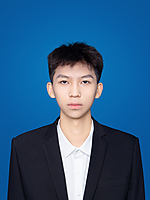
\includegraphics[width=1.72cm,height=2.38cm]{photo.png}}}}}\par

\begin{center}
    {\LARGE\bfseries \name} \\[0.42em]
    \faPhone\ \phone\hspace{0.25em}\textbar\hspace{0.25em}
    \href{mailto:\emaila}{\faEnvelope\ \emaila}\hspace{0.25em}\textbar\hspace{0.25em}
    \href{https://github.com/Botwwt}{\faGithub\ GitHub}\hspace{0.25em}\textbar\hspace{0.25em}
    \href{https://scholar.google.com/citations?user=tF1l1S0AAAAJ\&hl=zh-CN}{\faGraduationCap\ Scholar}
\end{center}

\section{个人介绍}
\begin{itemize}[leftmargin=1.25em, itemsep=0.08em, topsep=0.06em, parsep=0pt]
    \item 北京大学未来技术学院2027年入学直博生，导师马雷。现为大连理工大学数理基础科学专业 2023 级本科生，预计 2027 年 6 月毕业。学分绩：4.29/5.00；加权平均分：92.9/100；专业排名：7/99。
    \item 核心课程：数学分析（99）、高等代数（99）、概率论（99）、数据结构与算法（99）、最优化方法（99）、程序设计与算法（100）、解析几何（100）；英语成绩：CET-6 460，CET-4 522。
    \item 技术技能与研究兴趣：熟练掌握 Python、MATLAB、Java；熟练使用 PyTorch、Hugging Face Transformers、TRL、Unsloth 等工具，关注类脑计算、大语言模型、强化学习与长上下文建模。
\end{itemize}

\section{科研经历}
\noindent\textbf{北京大学} \quad 科研实习生 \hfill 2025年10月 -- 至今
\begin{itemize}[leftmargin=1.25em, itemsep=0.08em, topsep=0.06em, parsep=0pt]
    \item 围绕现有更新方式 BPTT 的时序信用分配问题开展研究，关注在线、具生物启发且低内存的局部学习规则，并验证其近似误差、稳定性与可扩展性。
\end{itemize}
\vspace{0.04em}

\noindent\textbf{中国科学院自动化研究所} \quad 科研实习生 \hfill 2024年12月 -- 至今
\begin{itemize}[leftmargin=1.25em, itemsep=0.08em, topsep=0.06em, parsep=0pt]
    \item 参与协同边缘缓存、长上下文恢复与无线通信大模型综述等研究，负责环境与训练流程搭建、实验组织、图表绘制、技术写作，并参与后续专利材料整理。
\end{itemize}
\vspace{0.04em}

\noindent\textbf{大连理工大学} \quad 本科科研 \hfill 2024年10月 -- 2025年3月
\begin{itemize}[leftmargin=1.25em, itemsep=0.08em, topsep=0.06em, parsep=0pt]
    \item 围绕取送货问题神经组合优化开展本科科研，完成模型设计、强化学习训练、基准构建、对比实验与论文撰写。
\end{itemize}
\vspace{0.04em}

\noindent\textbf{东方理工大学} \quad 科研实习生 \hfill 2025年8月 -- 2025年11月
\begin{itemize}[leftmargin=1.25em, itemsep=0.08em, topsep=0.06em, parsep=0pt]
    \item 阅读世界模型与视觉语言大模型相关文献，梳理代表性方法与技术路线。
\end{itemize}

\section{科研成果}
\noindent\textbf{Global Credit Assignment via Dynamical Criticality}
\begin{itemize}[leftmargin=1.15em, itemsep=0.02em, topsep=0.03em, parsep=0pt]
    \item \textbf{ICML 2026（CCF-A）已录用，第一作者}。北京大学。
    \item 现有 BPTT 虽精确但内存随序列长度线性增长且易梯度不稳，在线局部规则虽高效却常带来较大偏差；为此提出基于临界动力学的局部学习规则，通过空间长程惯量和时间长程关联将全局信用传播近似为局部可计算教学信号，并推导仅需常数级激活内存与 $\mathcal{O}(H)$ 辅助状态的闭式更新，在 RNN、ConvRNN 和 SNN 上验证其精度、稳定性与可扩展性。负责全文撰写和实验。[预印本可按需提供]
\end{itemize}
\vspace{0.03em}

\noindent\textbf{Decision-Making Large Language Model for Wireless Communication: A Comprehensive Survey on Key Techniques}
\begin{itemize}[leftmargin=1.15em, itemsep=0.02em, topsep=0.03em, parsep=0pt]
    \item \textbf{IEEE COMST 2025 已发表（IF 46.7，Q1），第三作者}。中科院自动化所。
    \item 针对现有综述对通信场景训练数据与决策流程梳理不足的问题，系统总结无线通信中决策型大语言模型的数据构建、架构适配、推理控制、多智能体协同与开放问题，梳理任务建模、训练范式与评测维度；独立撰写数据构建、架构适配和开放挑战等核心章节，负责全文技术图示绘制。 \href{https://ieeexplore.ieee.org/document/11180008/}{[IEEE Xplore]}
\end{itemize}
\vspace{0.03em}

\noindent\textbf{Cooperative Edge Caching with Large Language Model in Wireless Networks}
\begin{itemize}[leftmargin=1.15em, itemsep=0.02em, topsep=0.03em, parsep=0pt]
    \item \textbf{IEEE TMC 已录用（IF 9.2，Q1），第二作者（学生一作）}。中科院自动化所。
    \item 现有启发式缓存策略往往短视，DRL 方法又多依赖脆弱的数值状态/动作表示并在拓扑或流量变化下需要重训练；为此将协同边缘缓存形式化为大语言模型原生序列决策问题，构建多基站、多用户交互环境与文本到动作接口，完成 SFT+GRPO 训练并设计机会感知奖励，所得策略超过单基站单步穷举上限，并在不同用户规模、基站数量和请求分布下表现出良好泛化性；本人负责全文撰写和大部分实验。 \href{https://arxiv.org/abs/2602.13307}{[arXiv]} \href{https://github.com/gracefulning/CoopLLM-Cache}{[Code]}
\end{itemize}
\vspace{0.03em}

\noindent\textbf{LinearARD: Linear-Memory Attention Distillation for RoPE Restoration}
\begin{itemize}[leftmargin=1.15em, itemsep=0.02em, topsep=0.03em, parsep=0pt]
    \item \textbf{NeurIPS 2026（CCF-A）已录用，共一第三}。中科院自动化所。
    \item 现有 RoPE 缩放方法常破坏短上下文能力，CPT 成本高且易遗忘，已有恢复方法又多采用隐藏态匹配，难以精确校正注意力中的位置失真；为此提出 LinearARD，通过对齐原生 RoPE 教师与缩放 RoPE 学生的行级稠密自关系实现长上下文恢复蒸馏，并创新推导精确的线性内存 KL 散度核，在 LLaMA2-7B 4K$\to$32K 设定下仅用 4.25M Token 即可恢复 98.3\% 的短上下文基准性能；本人负责全文撰写。 \href{https://arxiv.org/abs/2604.00004}{[arXiv]} \href{https://github.com/gracefulning/LinearARD}{[Code]}
\end{itemize}
\vspace{0.03em}

\noindent\textbf{MC-TRCM: Observation-Aware Recursive Fusion for Incomplete Mobile and Wearable Mental-Health Feature Views}
\begin{itemize}[leftmargin=1.15em, itemsep=0.02em, topsep=0.03em, parsep=0pt]
    \item \textbf{ICONIP 2026（CCF-C）已录用，第一作者}。大连理工大学。
    \item 面向移动与可穿戴心理健康数据中异步、缺失的多源特征视图，提出 MC-TRCM，将各特征源独立编码并显式融入缺失信息，通过共享--私有潜变量、任务条件融合与递归预测实现多任务建模；在 DepreST-CAT 和 PSYCHE-D 的六项任务上取得领先或有竞争力的结果。 \href{https://github.com/Botwwt/MC-TRCM}{[Code]}
\end{itemize}
\vspace{0.03em}

\noindent\textbf{Cluster-Aware Attention-Based Deep Reinforcement Learning for Pickup and Delivery Problems}
\begin{itemize}[leftmargin=1.15em, itemsep=0.02em, topsep=0.03em, parsep=0pt]
    \item \textbf{\textit{Applied Intelligence} 大修（IF 3.4，Q2），第一作者}。大连理工大学。
    \item 现有 PDP 深度强化学习方法多在平坦图上隐式处理配对与先后约束，或依赖推理期协同搜索换取性能，导致结构利用不足且时延较高；为此提出 CAADRL，将全局自注意力、簇内注意力与动态双解码器结合，显式利用聚类结构求解取送货问题，在多个聚类基准数据集上取得领先性能，并较协同搜索基线显著降低推理时延。负责主实验和大部分撰写。 \href{https://arxiv.org/html/2603.10053v1}{[arXiv]} \href{https://github.com/Botwwt/CluPDTSP}{[Code]}
\end{itemize}

\section{荣誉奖项}
\begin{itemize}[leftmargin=1.25em, itemsep=0.025em, topsep=0.05em, parsep=0pt]
    \item \makebox[7em][l]{2026年06月} Kaggle BirdCLEF+ 2026 \textbf{铜牌}
    \item \makebox[7em][l]{2026年03月} Kaggle March Machine Learning Mania 2026 \textbf{铜牌}
    \item \makebox[7em][l]{2026年02月} 美国大学生数学建模竞赛（MCM）\textbf{Meritorious Winner（M奖）}
    \item \makebox[7em][l]{2025年11月} 全国英语翻译大赛 \textbf{国家二等奖}
    \item \makebox[7em][l]{2024年12月} 辽宁省级大创项目主力队员
    \item \makebox[7em][l]{2024年11月} 亚太地区大学生数学建模竞赛 \textbf{国家一等奖}
    \item \makebox[7em][l]{2024年09月} 全国大学生数学建模竞赛 \textbf{省级一等奖}
    \item \makebox[7em][l]{2024年01月} 美国大学生数学建模竞赛（MCM）\textbf{Honorable Mention}
\end{itemize}

\section{学术服务与活动}
\begin{itemize}[leftmargin=1.25em, itemsep=0.025em, topsep=0.05em, parsep=0pt]
    \item \textbf{学术审稿}：担任国际期刊 \textit{Journal on Wireless Communications and Networking}（JCR Q3）审稿人。
    \item \textbf{竞赛平台}：Kaggle 专家（Competitions Expert）。
    \item \textbf{学术交流}：参与新加坡国立大学暑期学术交流项目。
\end{itemize}

\end{document}
